\section{Comandos de ejecuci\'on y rutas}
\label{app:commands}

\subsection{Compilacion}

\begin{lstlisting}[language=bash]
cd /home/lostwin/Documentos/Sublime-Data/2026-I/MACRODATOS/Final-Macrodatos
make build
\end{lstlisting}

\subsection{Ejecucion mononodo}

\begin{lstlisting}[language=bash]
cd /home/lostwin/Documentos/Sublime-Data/2026-I/MACRODATOS/Final-Macrodatos
time make run-all
\end{lstlisting}

Esta ejecucion usa por defecto:

\begin{lstlisting}[language=bash]
SPARK_MASTER=local[*]
INPUT=file:///.../Final-Macrodatos/data/dataset_vf_3.csv
OUTPUT=file:///.../Final-Macrodatos/output
\end{lstlisting}

\subsection{Ejecucion multimodo sobre YARN}

\begin{lstlisting}[language=bash]
/opt/spark/bin/spark-submit \
  --class mdjm.Main \
  --master yarn \
  --conf spark.executor.instances=3 \
  --conf spark.dynamicAllocation.enabled=false \
  --conf spark.executor.cores=1 \
  --conf spark.executor.memory=512m \
  --conf spark.executor.memoryOverhead=384 \
  --conf spark.sql.shuffle.partitions=4 \
  /tmp/arbitrios-mdjm.jar \
  hdfs:///mdjm/input/dataset_vf_3.csv \
  hdfs:///mdjm/output_3nodes_verify_20260707_2325 \
  all
\end{lstlisting}

\subsection{Verificacion de salidas en HDFS}

\begin{lstlisting}[language=bash]
hdfs dfs -ls -R /mdjm/output_3nodes_verify_20260707_2325
hdfs dfs -cat /mdjm/output_3nodes_verify_20260707_2325/metrics/regression_metrics.json/part-*
hdfs dfs -cat /mdjm/output_3nodes_verify_20260707_2325/metrics/classification_metrics.json/part-*
hdfs dfs -cat /mdjm/output_3nodes_verify_20260707_2325/queries/query1_groupby_periodo.json/part-*
hdfs dfs -cat /mdjm/output_3nodes_verify_20260707_2325/queries/query2_top_predios_2025.json/part-* | head
\end{lstlisting}

\subsection{Salidas adjuntas en el proyecto del informe}

Para facilitar la revision en Overleaf, se adjuntan las salidas livianas en la carpeta \texttt{salidas/}:

\begin{itemize}
    \item \texttt{salidas/queries/}: JSON de las dos consultas Spark SQL.
    \item \texttt{salidas/metrics/}: metricas de regresion y clasificacion.
    \item \texttt{salidas/loss\_curves/}: puntos de las curvas de perdida de MLPRegressor y SVRegressor.
\end{itemize}

Las tablas completas \texttt{contribuyentes.json} y \texttt{emisiones.json}, asi como el CSV de entrada, se mantienen como entregables del proyecto por fuera del PDF debido a su mayor tamano.

\section{Capturas complementarias}

\begin{figure}[H]
    \centering
    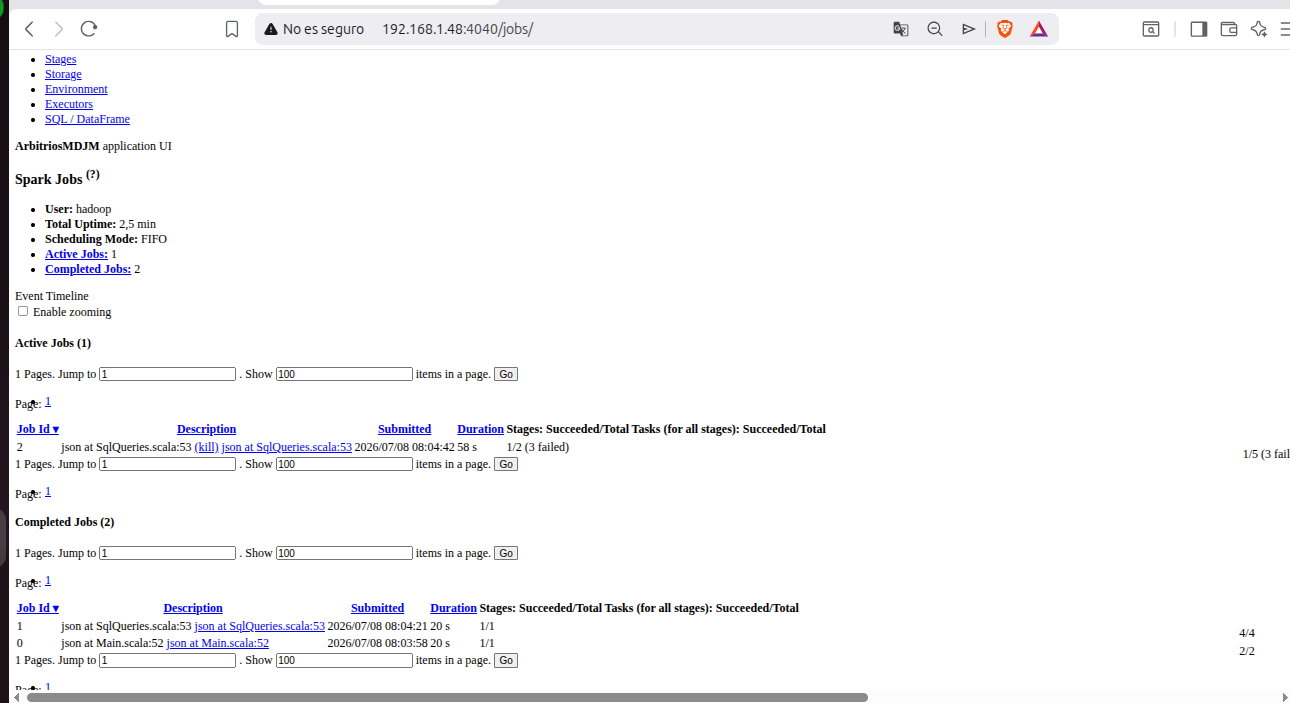
\includegraphics[width=\textwidth]{ImgMultiNodo/SPARKUISQL.png}
    \caption{Spark UI durante la ejecucion de consultas SQL en el cluster.}
    \label{fig:spark-ui-sql}
\end{figure}

\begin{figure}[H]
    \centering
    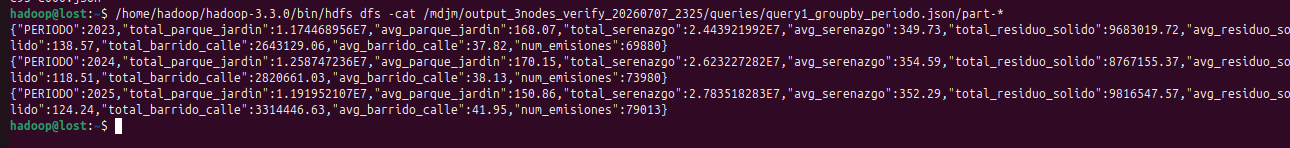
\includegraphics[width=\textwidth]{ImgMultiNodo/Query1_Resultado_Head.png}
    \caption{Salida JSON de la consulta 1 en HDFS.}
    \label{fig:query1-head}
\end{figure}

\begin{figure}[H]
    \centering
    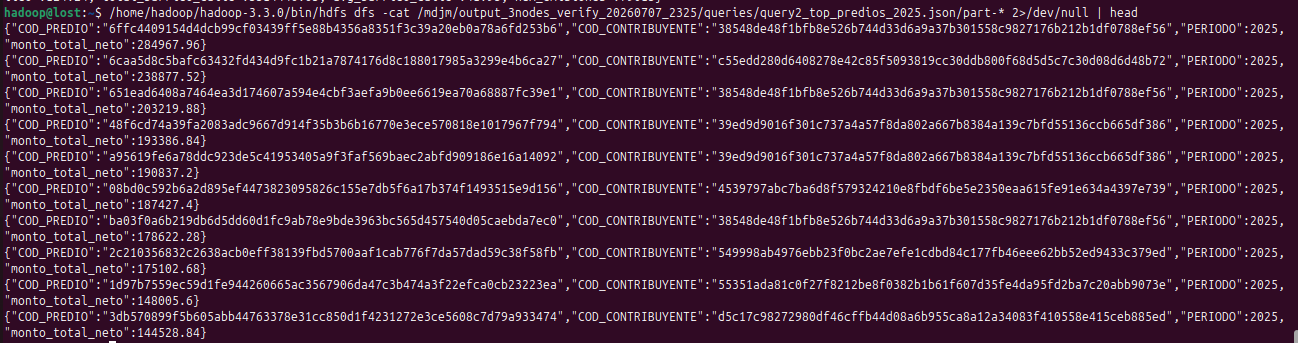
\includegraphics[width=\textwidth]{ImgMultiNodo/Query2_resultado_Head.png}
    \caption{Salida JSON de la consulta 2 en HDFS.}
    \label{fig:query2-head}
\end{figure}

\section{Archivos Scala adjuntos}
\label{app:scala}

Los archivos fuente fueron copiados dentro de este proyecto de informe en la ruta \texttt{codigo/mdjm/}. A continuacion se listan los archivos principales que implementan cada requerimiento:

\begin{itemize}
    \item \texttt{codigo/mdjm/ETL.scala}
    \item \texttt{codigo/mdjm/SqlQueries.scala}
    \item \texttt{codigo/mdjm/FeaturePipeline.scala}
    \item \texttt{codigo/mdjm/Main.scala}
    \item \texttt{codigo/mdjm/MetricsWriter.scala}
    \item \texttt{codigo/mdjm/mlp/MLPRegressor.scala}
    \item \texttt{codigo/mdjm/svr/SVRegressor.scala}
    \item \texttt{codigo/mdjm/classification/RFAndMLPClassification.scala}
\end{itemize}

\subsection{Fragmento ETL}
\lstinputlisting[language=scala,firstline=1,lastline=95]{codigo/mdjm/ETL.scala}

\subsection{Consultas SQL}
\lstinputlisting[language=scala,firstline=1,lastline=65]{codigo/mdjm/SqlQueries.scala}

\subsection{Orquestador principal}
\lstinputlisting[language=scala,firstline=1,lastline=110]{codigo/mdjm/Main.scala}
